\section{Introduzione agli strumenti usati}
Prima di addentrarci negli aspetti più teorici è bene trattare gli strumenti
computazionali usati durante la fase di sviluppo.\\
Dal punto di vista dei linguaggi di programmazione si sono usati:
\begin{itemize}
  \item \textbf{\Cplusplus}, per l'implementazione delle strutture dati e degli
  algoritmi
  \item \textbf{Python}, per la creazione della struttura a partire dal
  pannello in input e per gestire l'intera pipeline di sperimentazione,
  partendo dal \textit{preprocessing} dell'input fino alla produzione dei
  grafici al termine della computazione
\end{itemize}
Nel dettaglio la costruzione della \textbf{RLPBWT}, i cui
singoli step verranno approfonditi nel corso del capitolo, si articola nel
seguente modo: 
\begin{enumerate}
  \item \textit{\textbf{input:}} pannello binario generato tramite
  \textbf{MaCS}
  \item \textbf{opzionale:} produzione dell'\textbf{SLP} del pannello
  \item \textbf{step intermedio:} estrazione dal pannello in input di un
  pannello di query di grandezza selezionata dall'utente e costruzione della
  struttura dati  
  \item \textbf{opzionale:} serializzazione della struttura dati
  \item \textit{\textbf{output:}} file contenente i risultati dei match
\end{enumerate}
Si specifica che per il file di output si è mantenuto lo stesso formato
utilizzato da Durbin nella sua implementazione della \textbf{PBWT}
\cite{durbin_gh}. Tale formato prevede, per facilitarne il parsing, un
\texttt{tsv} (\textit{tab-separated values}) con le seguenti colonne:
\begin{enumerate}
  \item colonna semplicemente indicante che si ha un \textit{MATCH}
  \item l'indice della query di cui si annota il match
  \item l'indice dell'aplotipo per cui si ha il match
  \item l'indice della colonna da cui parte il match
  \item l'indice della colonna in cui termina il match
  \item la lunghezza del match
\end{enumerate}
Un esempio è visualizzabile alla listing \ref{lst:pbwtres}.
\subsection{MaCS}
\textbf{RIVEDERE!}\\
\textbf{MaCS} \cite{macs}, sviluppato da Gary K. Chen, è un simulatore di
\textit{processi coalescenti}, basati sulla \textbf{teoria della
  coalescenza}. Tale teoria è un modello di come gli alleli campionati da una
popolazione possano essere originati da un antenato comune. Il tool simula
genealogie spaziali tra i cromosomi sfruttando processi Markoviani.\\
Nel dettaglio il lavoro è fortemente ispirato dai risultati di Wiuf e Hein
\cite{wiuf}, che per primi proposero un algoritmo basato sulla costruzione e
sulla memorizzazione di un \textbf{ancestral recombination graph
  (\textit{ARG})}.\\
Chen stesso segnala le seguenti differenze con l'algoritmo di Wiuf e Hein:
\begin{itemize}
  \item gli eventi di ricombinazione si verificano solo sulla geneologia locale
  nella posizione attuale sulla sequenza invece che in qualsiasi altro punto
  dell'\textit{ARG}, ma possono unirsi a qualsiasi lignaggio sull'ARG compresi
  quelli non sulla geneologia locale (ad esempio un arco non ancestrale)
  \item i tempi di attesa (ovvero la distanza tra le ricombinazioni sulla
  sequenza) sono calcolati in modo esponenziali con intensità basata sulla
  lunghezza dell'arco della geneologia locale invece della lunghezza
  \textit{ARG}
  \item l''algoritmo è detto dell'$n$-esimo ordine Markoviano, dove $n$ è basato
  sui parametri inserito dall'utente
\end{itemize}
L'autore ricorda che queste modifiche rendono l'algoritmo sostanzialmente più
efficiente del Wiuf e Hein con poca perdita di precisione. \\
Dal punto di vista pratico l'esecuzione di \textit{MaCS} produce i pannelli
binari, da intendersi come pannelli di aplotipi, che verranno poi studiati
tramite la \textit{PBWT} e la \textit{RLPBWT}. Tali pannelli presentano:
\begin{itemize}
  \item un header, con informazioni in merito al comando usato e al seed
  \item una riga per ogni sito, con prima alcune informazioni in merito a come è
  stato prodotto il dato e poi la sequenza di valori binari, uno per ogni sample
  \item un footer, con ulteriori informazioni, tra cui le dimensioni del
  pannello 
\end{itemize}
Quindi, trascurando le varie informazioni aggiuntive, il pannello è
\textbf{trasposto} rispetto a quanto studiato dalla \textit{PBWT} e dalla
\textit{RLPBWT}. Questa però risulta essere una comodità in quanto, leggendo
iterativamente il file, si legge di volta in volta la $i$-esima colonna, ovvero
quanto serve per la costruzione della struttura dati.\\
Per capire meglio come venga prodotto un pannello tramite questo strumento,
analizziamo un semplice esempio:
\begin{shaded}
  \begin{minted}{bash}
    ./macs 5 3000 -t 0.001 -r 0.001
  \end{minted}
\end{shaded}
\noindent
Dove:
\begin{itemize}
  \item $5$ è il numero di sample richiesto, ovvero il numero di sequenze che
  il software simulerà
  \item $3000$ è la lunghezza in paia-basi della regione genomica su cui
  verranno simulate le $5$ sequenze
  \item \texttt{-t} $0.001$ segnala il \textit{mutation rate} per ogni sito,
  ovvero la frequenza di \textit{nuove mutazioni} per un sito nel tempo 
  \item \texttt{-r} $0.001$ segnala il \textit{recombination rate} per ogni
  sito, ovvero la frequenza di \textit{ricombinazioni geniche}, che sono i
  processi per i quali si ottengono nuove combinazioni di alleli a partire da un
  \textit{genotipo}, per un sito nel tempo 
\end{itemize}
Il risultato, dove si noti vengono selezionati 4 siti dopo la simulazione, del
comando appena descritto è visualizzabile alla listing \ref{lst:macs}.\\ 
\textbf{MANCA SIGNIFICATO DEGLI ``HEADER'' DI OGNI SITE NEL RISULTATO.}
\subsection{SDSL}
La libreria più utilizzata nel progetto, come anche in diverse sue dipendenze, è
\textbf{Succinct Data Structure Library (\textit{SDSL})} \cite{sdsl}. Questa
libreria, scritta in \Cplusplus 11, fornisce diverse implementazioni riguardanti
strutture dati succinte, come i già citati, nella sezione \ref{bvsec},
\textbf{bitvectors}.\\ 
Nel dettaglio, in questo progetto, \textit{SDSL} è stata usata per:
\begin{itemize}
  \item gli \textbf{sparse bitvectors}, il cui uso specifico verrà specificato
  più avanti nel capitolo
  \item i cosiddetti \textbf{int vectors}, ovvero vettori di interi memorizzati
  in modo efficiente
  \item le funzioni di atte a gestire le \textbf{serializzazioni} delle
  strutture dati implementate
  \item stimare, in certi casi, lo \textbf{spazio in memoria} richiesto per le
  varie strutture 
\end{itemize}
\subsection{BigRePair e ShapedSlp}
Come introdotto alla sezione \ref{slpsec}, una delle varianti della
\textbf{RLPBWT}, richiede l'uso, estremamente vantaggioso dal punto di vista
della memoria occupata, degli \textbf{SLP}.\\
Da un punto di vista implementativo, l'oggetto contenente l'\textit{SLP} del
pannello viene costruito ed interrogato mediante l'uso della libreria
\textbf{ShapedSlp} \cite{shapedslp}, implementazione dei risultati ottenuti da
Gagie et al. \cite{slpgagie}. Inoltre, tale libreria basa il suo funzionamento
sull'uso di un'altra libreria, detta \textbf{BigRePair} \cite{bigrepair}, che
implementa i quanto studiato da Gagie et al. \cite{rpair} in merito alla
compressione, via uso di grammatiche, di file con frequenti ripetizioni (come
possono essere, nel nostro caso, pannelli binari di aplotipi).\\
In termini di pipeline si procede quindi:
\begin{enumerate}
  \item generando la \textit{grammatica} tramite \textit{BigRePair}, che accetta
  come file di input un file \texttt{txt} ``raw'' ma anche un file in formati
  più standard come i \textit{FASTA}
  \item generando l'\textit{SLP} tramite \textit{ShapedSlp} specificatamente a
  partire dai risultati di \textit{BigRePair} (si segnala che la libreria
  accetta anche input prodotti tramite altri tool che non verranno qui
  approfonditi) 
\end{enumerate}
\subsubsection{Compressione del panel}
I tool appena citati assumono un input ``monodimensionale'', ovvero una singola
sequenze lineare. Nel nostro caso l'input era invece un file \texttt{.macs} con
rappresentato il pannello trasposto. Nel dettaglio, assumendo di avere il
pannello come nella listing \ref{lst:macs} (pannello al quale sono giù state
estratte le query), si avrebbe, isolando:
\[
  X=\left[
    \begin{matrix}
      0 & 0 & 1 & 0 & 0\\
      1 & 1 & 1 & 0 & 1\\
      0 & 1 & 1 & 1 & 1\\
      0 & 0 & 0 & 1 & 0
    \end{matrix}
  \right]
\]
Dove però come detto le righe sono i siti e le colonne i sample. Per ottenere
l'\textit{SLP} biosgna quindi, in primis, trasporre la matrice:
\[
  X^T=\left[
    \begin{matrix}
      0 & 1 & 0 & 0\\
      0 & 1 & 1 & 0\\
      1 & 1 & 1 & 0\\
      0 & 0 & 1 & 1\\
      0 & 1 & 1 & 0
    \end{matrix}
  \right]
\]
Per procedere ulteriormente bisogna però ricordare che sull'\textit{SLP} si avrà
necessità di effettuare \textit{LCE query} che però, si anticipa, nel nostro
pannello, devono essere fatte tra due righe da destra a sinistra (a differenza
di quanto visto nel caso standard dove si confrontavano prefissi comuni). Ad
esempio, prendendo la seconda e la terza riga, avremmo una \textit{LCE query}
lunga 3, terminante nella prima colonna esclusa:
\begin{figure}[H]
  \centering
  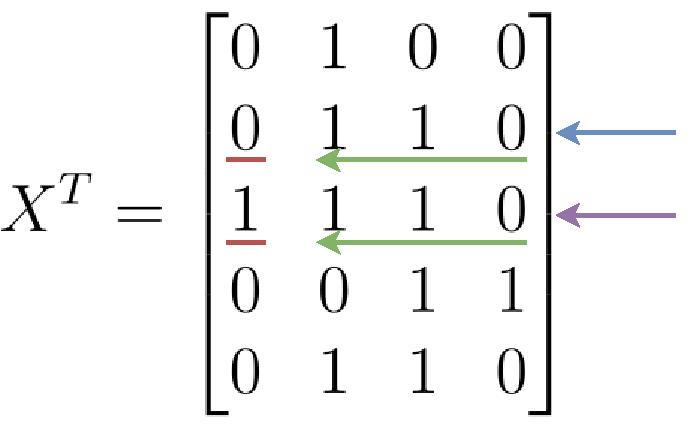
\includegraphics[scale = 0.38]{img/slppanel.pdf}
\end{figure}
Per rendere possibile questa operazione quindi il pannello deve essere sia
salvato come un'unica riga, per ottenerne l'\textit{SLP}, che ``da destra a
sinistra'', per permettere le \textit{LCE query}. Si procede quindi concatenando
ogni riga, selezionandole consecutivamente e leggendone i singoli elementi da
destra a sinistra ottenendo, con colorate gli stessi risultati della query fatta
sopra:
\[0010\,\,{\color{nordgreen}011}{\color{nordred}0}\,\,
  {\color{nordgreen}011}{\color{nordred}1} \,\,1100\,\,0110\]
\textit{Si noti che qui si sono segnalate le varie righe con uno spazio ma solo
  per praticità ``visiva''.}
\subsection{Snakemake}
\textbf{PARTE DA FARE UNA VOLTA STABILITA LA PIPELINE FINALE}